\chapter{背景知識}

%2.1
\section{i18n工具相關知識}

%2.1.1
\subsection{國際化}
國際化(Internationalization)\cite{internationalization},簡寫為i18n,其中18代表i和n之間的18個英文字母。國際化是開發軟體時,將軟體本身和特定語言、地區脫鉤的一個過程,除了可以滿足不同的地區、文化的大眾需求,移植軟體到不同的語言環境時,也不須改變內部程式的實作。

%2.1.2
\subsection{自動化驗收測試}
驗收測試(Acceptance Testing)\cite{se},是一種站在使用者的立場,去檢驗一個真實存在的系統,是否滿足使用者需求與預期的測試方法。

而透過撰寫自動化測試腳本\cite{AT},如今我們可以執行更符合成本,且更加精確的自動化驗收測試。改善了過往手動執行驗收測試時,存在的人為操作誤差、系統問題無法即時呈現、成本較高等問題。

\hspace*{\fill} \\
\\ \hspace*{\fill} \\
%2.1.3
\subsection{XPath}
XPath\cite{xpath},全名為 XML Path Language,可以用來定位XML檔案中某節點所處在的位置。在使用Robot Framework撰寫的網頁自動化驗收測試中,我們便時常需要藉助XPath,去找到並確定畫面上某元件的位置,以對其狀態進行測試。

%2.1.4
\subsection{JSON格式翻譯檔在前端框架中的運作}
JSON格式\cite{json}的多國語言翻譯檔,其結構是由撰寫者自定義的‘Key’,對應網頁上所要呈現的翻譯詞‘Value’所構成;而一個Value,可以使用一個或以上的Key階層結構定位。例如:在英文JSON翻譯檔下,i18n這個Value,其Key值是“EXAMPLE.INTERNATIONALIZATION”(如圖~\ref{angular-translate英文JSON翻譯檔})。

而在前端框架中,若我們要透過JSON格式的多國語言翻譯檔,進行多國語言網頁翻譯,則必須使用第三方套件;在此以AngularJS\cite{angularjs}搭配第三方套件angular-translate\cite{angular-translate}為例,將英文網頁翻譯成中文網頁。首先,將待翻譯詞定義在JSON格式的英文翻譯檔(如圖~\ref{angular-translate英文JSON翻譯檔}),以及其中文翻譯定義在JSON格式的中文翻譯檔(如圖~\ref{angular-translate中文JSON翻譯檔}),並在HTML內的需翻譯詞處加上對應的標記(如圖~\ref{HTML翻譯標記})。之後,AngularJS便會根據當前網頁的語言-中文,以及待翻譯元件標記處的Key值-“EXAMPLE.INTERNATIONALIZATION”,去中文的JSON翻譯檔查找該Key值對應的Value,最後將找到的翻譯詞-「國際化」顯示於網頁上。

\hspace*{\fill} \\
\\ \hspace*{\fill} \\
\begin{figure}[H]
    \centering
    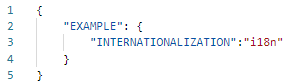
\includegraphics[width= .6\textwidth]{../論文截圖/angular-translate英文JSON翻譯檔.png}
    \caption{英文JSON翻譯檔示例}
    \label{angular-translate英文JSON翻譯檔}
\end{figure}

\hspace*{\fill} \\
\begin{figure}[H]
    \centering
    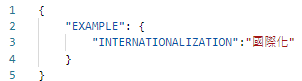
\includegraphics[width= .6\textwidth]{../論文截圖/angular-translate中文JSON翻譯檔.png}
    \caption{中文JSON翻譯檔示例}
    \label{angular-translate中文JSON翻譯檔}
\end{figure}

\hspace*{\fill} \\
\begin{figure}[H]
    \centering
    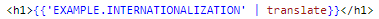
\includegraphics[width= .8\textwidth]{../論文截圖/HTML翻譯標記.png}
    \caption{於HTML內加入翻譯標記}
    \label{HTML翻譯標記}
\end{figure}

\hspace*{\fill} \\
\\ \hspace*{\fill} \\
\\ \hspace*{\fill} \\
%2.2
\section{Robot Framework}
Robot Framework\cite{rf}\cite{rfguide}是一個開源的框架語言,可以用來執行自動化驗收測試或機器人自動化,核心框架是由Python\cite{python}編寫而成,測試者可以使用Python或Java擴充其函式庫。其特色是擁有簡單的語法,以及容易理解的原生關鍵字(Keyword),測試者可以視需求使用並包裝成更接近自然語言的關鍵字。

\subsection{Robot Framework關鍵字}
Robot Framework透過許多的關鍵字(Keyword)來構成一份測試腳本,關鍵字分為兩種:Robot Framework的原生關鍵字,以及使用者自己定義的關鍵字。Robot Framework的原生關鍵字可以透過引入Library來使用,能夠達成絕大多數對網頁上元件的基本操作,例如:Click Element、Open Browser;或是一些基礎的邏輯判斷,例如:Should Be Equal;以及一些對變數的設定與印出,例如:Set Variable、Log。

而使用者自定義的關鍵字,則是根據當下測試案例(Test Case)的需要,將一或多個原生關鍵字包裝成為更具體、易讀、能夠描述當下測試動作的關鍵字;例如:想使用測試腳本去點擊Microsoft官方網頁上的「支援」按鈕,則可撰寫“Click Support Button On Microsoft Page”這個自定義的關鍵字,裡面包裝了原生關鍵字“Open Browser”以及“Click Element”,分別執行打開瀏覽器和點擊按鈕的動作。

此外,實際使用上,隨著每個人或組織的要求程度不同,包裝原生關鍵字成為自定義的關鍵字也會有嚴謹程度上的不同。但是Robot Framework本身對這部分並沒有強制的規定,是很自由的。

\subsection{Robot Framework測試腳本}
一個Robot Framework 的測試腳本基本上由四個區塊構成,分別是:
\begin{itemize}
    \item[1.]Settings: 包含了使用到的library與resource file,也可以將Test Setup(測試腳本執行前要做的動作)、Test Teardown(測試腳本執行後要做的動作)定義於此。
    \item[2.]Test Cases: 在此測試者可以為各項想要驗證的使用者需求,撰寫核心的測試腳本
    \item[3.]Keywords: 如果測試腳本使用並非Robot Framework的原生關鍵字,或未被定義於其他resource file中,測試者可以在此處撰寫出新的關鍵字去達到測試目的。
    \item[4.]Variables: 測試者可以在此處定義測試案例需要用到的Global變數。 
\end{itemize}

\subsection{Robot Framework測試報表}
在測試腳本運行結束後,Robot Framework會產生出一份測試報表,記錄了整體的執行狀況,包含測試通過或失敗、腳本執行時間,並透過可展開的階層式圖表,方便測試者去追蹤到當前出現問題的關鍵字,進而修復錯誤。

\subsection{Robot Framework Listener}
Robot Framework提供了Listener\cite{rfguide}的介面,用以接收測試不同時期的資訊,並可以實作此介面,在測試腳本執行的不同時期做出額外的反應;例如實作end\_suite()函式,在測試結束後開啟一詞多譯UI,供使用者選擇。

此外,Robot Framework的Listener分為Version2和Version3兩種版本;以本論文來說,使用到的是版本Version2,必須在實作Listener處加上:
\begin{lstlisting}[language={python}]
ROBOT_LISTENER_API_VERSION=2
\end{lstlisting}
以供系統辨認要實作的Listener版本。而為了讓系統在測試執行時呼叫Listener,在執行測試腳本前必須設定- -listener組態,來指定需要使用到哪些自定義的Listener。

%2.3
\section{第一版i18n的系統介紹}
以下將分成第一版i18n的系統架構、執行流程,以及執行測試腳本時會產生一詞多譯問題的緣由,來說明第一版i18n工具的相關背景知識。

%2.3.1
\subsection{第一版i18n的系統架構}
第一版i18n的系統類別圖(如圖~\ref{1stI18nClassDiagram}),包含了3個 Robot Framework原生類別: RobotFramework、Listener、和Report;第一版i18n所設計的5個系統類別 :I18nListener、MappingRoutesGenerator、I18nMap、I18nTrigger、Proxy,以及5個實作自Proxy\cite{proxy}類別的代理關鍵字類別: ShouldContainProxy、ElementTextShouldBeProxy、FindElementProxy、ListsShouldBeEqualProxy、ShouldBeEqualProxy。\cite{i18n}

\begin{figure}[H]
    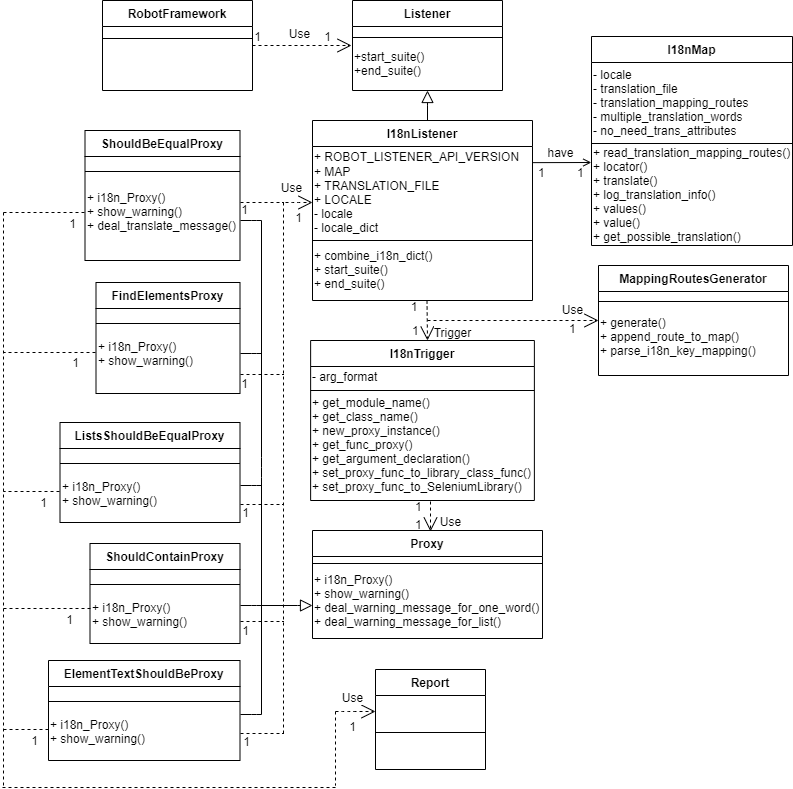
\includegraphics[width= 1.1\textwidth]{../UML/i18n class diagram-第一版正式版i18n class diagram.png}
    \caption{第一版i18n的系統類別圖}
    \label{1stI18nClassDiagram}
\end{figure}

I18nListener類別實作Listener類別,負責程式開始與結束時執行start\_suite()和end\_suite()的內容,並對MappingRoutesGenerator、I18nMap、I18nTrigger三個類別進行初始化的動作。I18nMap類別負責處理各個代理關鍵字類別透過I18nListener類別的呼叫,並將待翻譯詞做翻譯後回傳。I18nTrigger類別透過new\_proxy\_instance()函式建立各個代理關鍵字類別的實例;並使用set\_proxy\_func\_to\_library\_class\_func()、set\_proxy\_func\_to\_SeleniumLibrary()兩函式,將代理關鍵字類別的實作包裝於Robot Framework原生關鍵字之外,使每次呼叫關鍵字時,必先執行代理關鍵字的實作。MappingRoutesGenerator類別負責以英文JSON翻譯檔為基準,產生出翻譯路徑檔,讓測試腳本運行在其他語言環境下,可以根據此路徑,在所屬語言的JSON翻譯檔下找到正確的翻譯。Proxy類別提供了一個介面,讓實作Proxy類別的代理關鍵字類別可以根據各自的需要,去擴充內部的實作;其中,i18n\_Proxy()函式提供各代理關鍵字類別撰寫核心的功能。

%2.3.2
\subsection{第一版i18n的系統執行流程}
第一版i18n系統流程的Sequence Diagram(如圖~\ref{1stI18nSequenceDiagram}),在使用i18n工具執行測試腳本前,使用者必須於Red編輯器\cite{red}中的Additional Robot Framework arguments設定系統參數為-d out –L debug - -listener i18n/listeners/I18nListener.py:zh-TW,zh-TW代表當前語言為繁體中文-台灣(如圖~\ref{rfSysArgsSetting})。並且,使用此i18n工具的前提,必須建立在「使用者對於自己所提供的JSON翻譯檔,有充分的了解」,如此,當遭遇一詞多譯時,使用者才會明確知道在當下情況,什麼翻譯是正確的。(此前提套用到新版的i18n工具上亦然) 

\begin{figure}[H]
    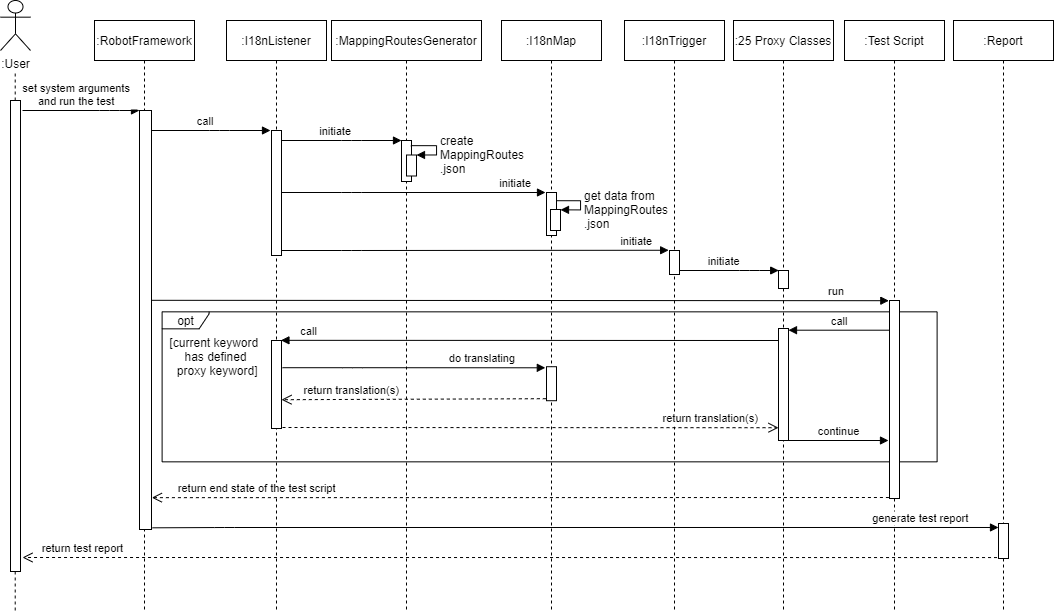
\includegraphics[width= 1.15\textwidth]{../UML/i18n sequence diagram-第一版i18n系統流程.png}
    \caption{第一版i18n的系統流程Sequence Diagram}
    \label{1stI18nSequenceDiagram}
\end{figure}

\begin{figure}[H]
    \centering
    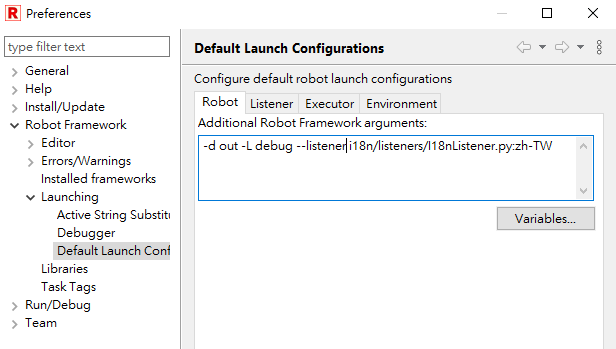
\includegraphics[width= 0.8\textwidth]{../論文截圖/3-1-3-1 設定系統參數.png}
    \caption{Robot Framework系統參數設定}
    \label{rfSysArgsSetting}
\end{figure}
測試執行時,系統會先去呼叫I18nListener類別並執行其實作。之後初始化MappingRoutesGenerator類別,藉由讀取由使用者自行提供的英文JSON格式翻譯檔(如圖~\ref{英文的JSON格式翻譯檔示例}),建立出一份由「待翻譯詞」和「Key階層」構成的翻譯路徑檔(如圖~\ref{翻譯路徑檔});例如待翻譯詞‘Support’,有兩種Key階層的路徑: “['SUPPORT']" 和 “['SUB\_BAR']['BLUE\_TITLE']['MICROSOFT\_SUPPORT']",代表‘Support’在多國語言網頁中,會在不同情境下被翻譯成兩種不同的詞彙。接著系統會依序初始化I18nMap、I18nTrigger,以及所有代理關鍵字類別。

\begin{figure}[H]
    \centering
    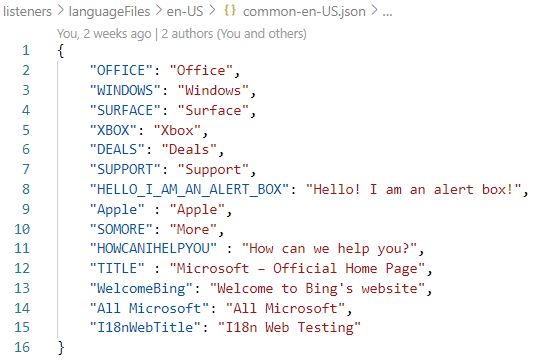
\includegraphics[width= .7\textwidth]{../論文截圖/3-1-3-2 JSON格式翻譯檔.png}
    \caption{英文的JSON格式翻譯檔示例}
    \label{英文的JSON格式翻譯檔示例}
\end{figure}

\begin{figure}[H]
    \centering
    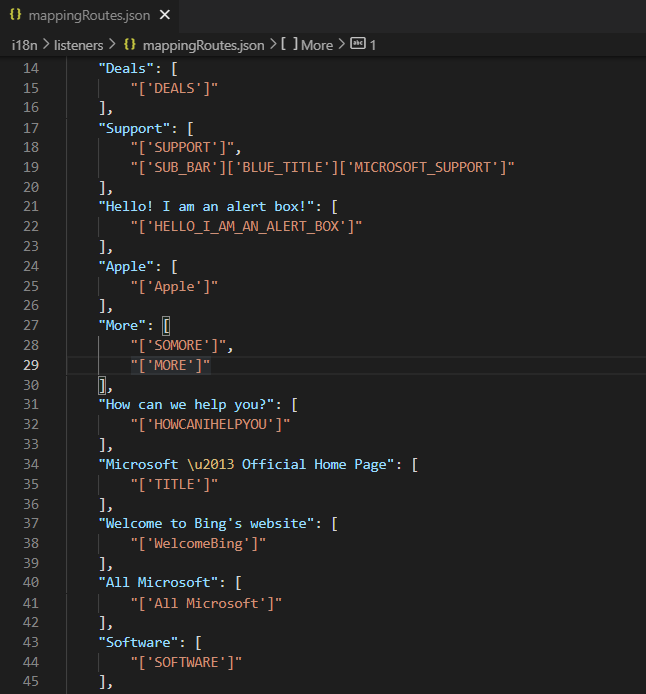
\includegraphics[width= .7\textwidth]{../論文截圖/3-1-3-3 翻譯路徑檔.png}
    \caption{翻譯路徑檔部分示例}
    \label{翻譯路徑檔}
\end{figure}
當執行完上述工作後,測試腳本才會正式開始執行;每當腳本運行到一個有定義代理的關鍵字,系統就會去呼叫對應的代理關鍵字物件,並執行翻譯邏輯。最後,當測試腳本執行結束,系統則會將一詞多譯的warning資訊顯示在報表上。

\hspace*{\fill} \\
\\ \hspace*{\fill} \\
\\ \hspace*{\fill} \\
%2.3.3
\subsection{產生一詞多譯問題的緣由}
執行多國語言網頁自動化驗收測試時,會產生「一詞多譯」問題的根本原因,源自於在前端的多國語言網頁設計中,可能必須根據當下網頁情況的不同,將同一個詞語,在不同語言的網頁上翻譯成為不同的詞。例如: 在Microsoft英文官方網頁上的‘Support’,在中文版網頁對應的不同頁面上,被分別翻譯為「支援」與「支援服務」。

此外,前端開發人員會隨著多國語言網頁的設計,產出一包JSON翻譯檔,裡面定義著不同語言之間,同一個詞語應該要被如何翻譯;並將此包JSON翻譯檔交給測試人員,以進行多國語言的網頁自動化驗收測試。

然而,對於測試人員而言,假如要驗證畫面上的一個元件,其text()屬性值是‘Support’的翻譯,在遭遇一詞多譯時,JSON檔卻只能告知‘Support’可能被翻譯成「支援」或「支援服務」;JSON檔內的Key階層對於測試人員而言並沒有太大的意義,因為測試腳本的撰寫是站在模擬使用者操作的角度,並不會把前端開發者的設計思維考慮進去。如此,就會造成多國語言網頁的一詞多譯特性,在測試人員進行自動化驗收測試的階段時,發生系統不知該如何選擇當下正確翻譯詞的問題。

第一版的i18n工具,在遭遇一詞多譯時,僅於測試報表上顯示warning資訊,提供待翻譯詞可能的翻譯有哪些;雖然成功呈現了系統目前有遭遇一詞多譯的問題,但尚未給出一個有效的解法。
